\documentclass[a4j,twocolumn]{jsarticle}

\usepackage[top=6.6truemm,bottom=15truemm,left=9truemm,right=9truemm]{geometry}
\usepackage[dvips,dvipdfmx]{graphicx}
\usepackage{mediabb}
\usepackage{bm}
\usepackage{comment}
\usepackage{amsmath}
\usepackage{amssymb}
\usepackage{subfigure}
\renewcommand{\baselinestretch}{0.85}

\title{Over-smoothing 防止のための層ごとに重み付けするSummarize-GNN}
\author{情報科学専攻~猪口研究室~
47020726~矢嶋 悠太 }
\date{}

\begin{document}
\maketitle

%%%%%%%%%%%%%%%%%%%%%%%%%%%%%%%%%%%%%%%%
\section{はじめに}
\label{sec_introduction}
\vspace{-1mm}
属性をもつ頂点と辺からなるグラフ構造は、SNSなど実世界の様々なデータを表現できる。
グラフの各頂点を高精度にクラス分類することは、SNSの各ユーザを適切なコミュニティに分類することに対応する。
近年、頂点の高精度なクラス分類のために、グラフを入力として、互いに属性が似ていたり、辺で結ばれている頂点同士が空間上の近い位置にマッピングされるように、各頂点をベクトル表現する、表現学習が注目されている。
頂点のベクトル表現が得られると、既存のクラス分類モデルにそのベクトル表現を入力するだけで、頂点のクラス分類が可能になる。
頂点のクラス分類精度を向上させる、質の高い頂点の表現を学習するために、近年は深層学習を用いた手法であるGraph~Neural~Network~(GNN)\cite{Kipf}\cite{Velickovic}が注目されている。

GNNは層数を適切に設定することで高い頂点の分類精度が得られる一方、より多層にすると分類精度が低下する。
GNNを多層化したときに、学習される頂点の表現の質が低下し、クラス分類精度が落ちる現象をOver-smoothingという。
本研究はOver-smoothingの課題を解決することを目的とする。


%%%%%%%%%%%%%%%%%%%%%%%%%%%%%%%%%%%%%%%%
\vspace{+1mm}
\subsection*{グラフの定義及び頂点のクラス分類}

グラフを$G=(V,E,X)$とする。ここで$V$は$n$個の頂点集合$\{1,\ldots,n\}$、$E$は頂点$v$から$u$への有向辺$e_{vu}$の集合である。
また、各頂点$v$がもつ属性$\bm{x}_v$は$a$次元のベクトルとし、全頂点の属性の集合を$X=\{ \bm{x}_1, \ldots, \bm{x}_n \}$とする。

グラフ$G$を入力とし、GNNモデルにより、全頂点のベクトル表現$H=\{\bm{h}_1, \ldots ,\bm{h}_n\}$を出力する。
$H$を入力とし、クラス分類モデルにより、全頂点のクラスラベルを予測する。
本研究では、既存のGNNモデル\cite{Kipf}\cite{Velickovic}よりも、頂点のクラス分類精度を向上させる質の高い$H$を出力するモデルを提案する。


%%%%%%%%%%%%%%%%%%%%%%%%%%%%%%%%%%%%%%%%
\section{近傍内の頂点の属性を集約するGNN}
\label{sec_gnn}

GNNは、$G$と層数$L$を入力とし、頂点$v$の表現$\bm{h}_v$を求める。\vspace{-6mm}
\begin{align}
  & \bm{h}_v^l = \text{Conv}(H^{l-1}, N(v)) = \sigma\left( W^l \sum_{u\in N(v)} w_{vu}^l\bm{h}_u^{l-1} \right) \label{eq_gnn1} \\
  & \bm{h}_v   = \bm{h}_v^L \label{eq_gnn2}
\end{align}
頂点$v$自身を含む、有向辺$e_{vu}$により$v$に接続されている頂点の集合$:\{v\} \cup \{u ~|~ e_{vu} \in E\}$を「$v$の1近傍内」と呼ぶ。
また、$\bm{h}_v^0$は属性$\bm{x}_v$、$\sigma(\cdot)$は活性化関数である。
$l-1$から$l$層に進む度、式(\ref{eq_gnn1})の畳み込み$\text{Conv}$により、頂点$v$の表現$\bm{h}_v^{l-1}$を$\bm{h}_v^{l}$に更新する。
各$l$層の$\text{Conv}$では以下を順に実行する。\vspace{-2mm}
\begin{itemize}
  \item[1.] $v$の1近傍内の各頂点$u\in N(v)$の表現を足し合わせる集約
  \item[2.] 行列$W^l$と活性化関数$\sigma(\cdot)$による線形及び非線形な変換\vspace{-2mm}
\end{itemize}
よって、Convを2回繰り返して得られる表現$\bm{h}_v^2$には、$v$の1近傍内である$u\in N(v)$の、更に1近傍内である$u' \in N(u)$の属性$\bm{x}_{u'}$が集約される。
つまり、$\bm{h}_v^2$には2近傍内の頂点$u'$の属性$\bm{x}_{u'}$が集約される。

式(\ref{eq_gnn2})より、GNNは$\text{Conv}$を層数$L$回繰り返して得られる、$L$近傍内の頂点の属性が集約された$\bm{h}_v^L$を$\bm{h}_v$として出力する。


\section{GNNの課題:Over-smoothingの原因の推察}
\label{sec_over_smoothing}

適切な層数$L_v^*$のGNNは質の高い表現を得ることができ、近年最高峰の分類精度を達成している\cite{Kipf}\cite{Velickovic}。
一方、GNNの層数$L$を$L_v^*$より大きくする程、表現$\bm{h}_v(=\bm{h}_v^L)$の質が低下し、その後のクラス分類精度も低下する現象をOver-smoothingと呼ぶ。

図\ref{fig_example1}の赤と青の破線で示すように、将来的に分類すべき頂点のクラスラベルが全て分かっている、という前提でOver-smoothingの原因を推察する。
グラフの中心にある$v$は1近傍内だけ集約すれば、自身と同ラベルの頂点の属性を全て集約できる。
端にある$u$はより遠くの近傍内を集約してようやく、自身と同ラベルの頂点の属性を全て集約できる。
つまり、頂点$v$ごとに適切な集約距離$L_v^*$は異なる。

\begin{figure}[!h]
  \centering
  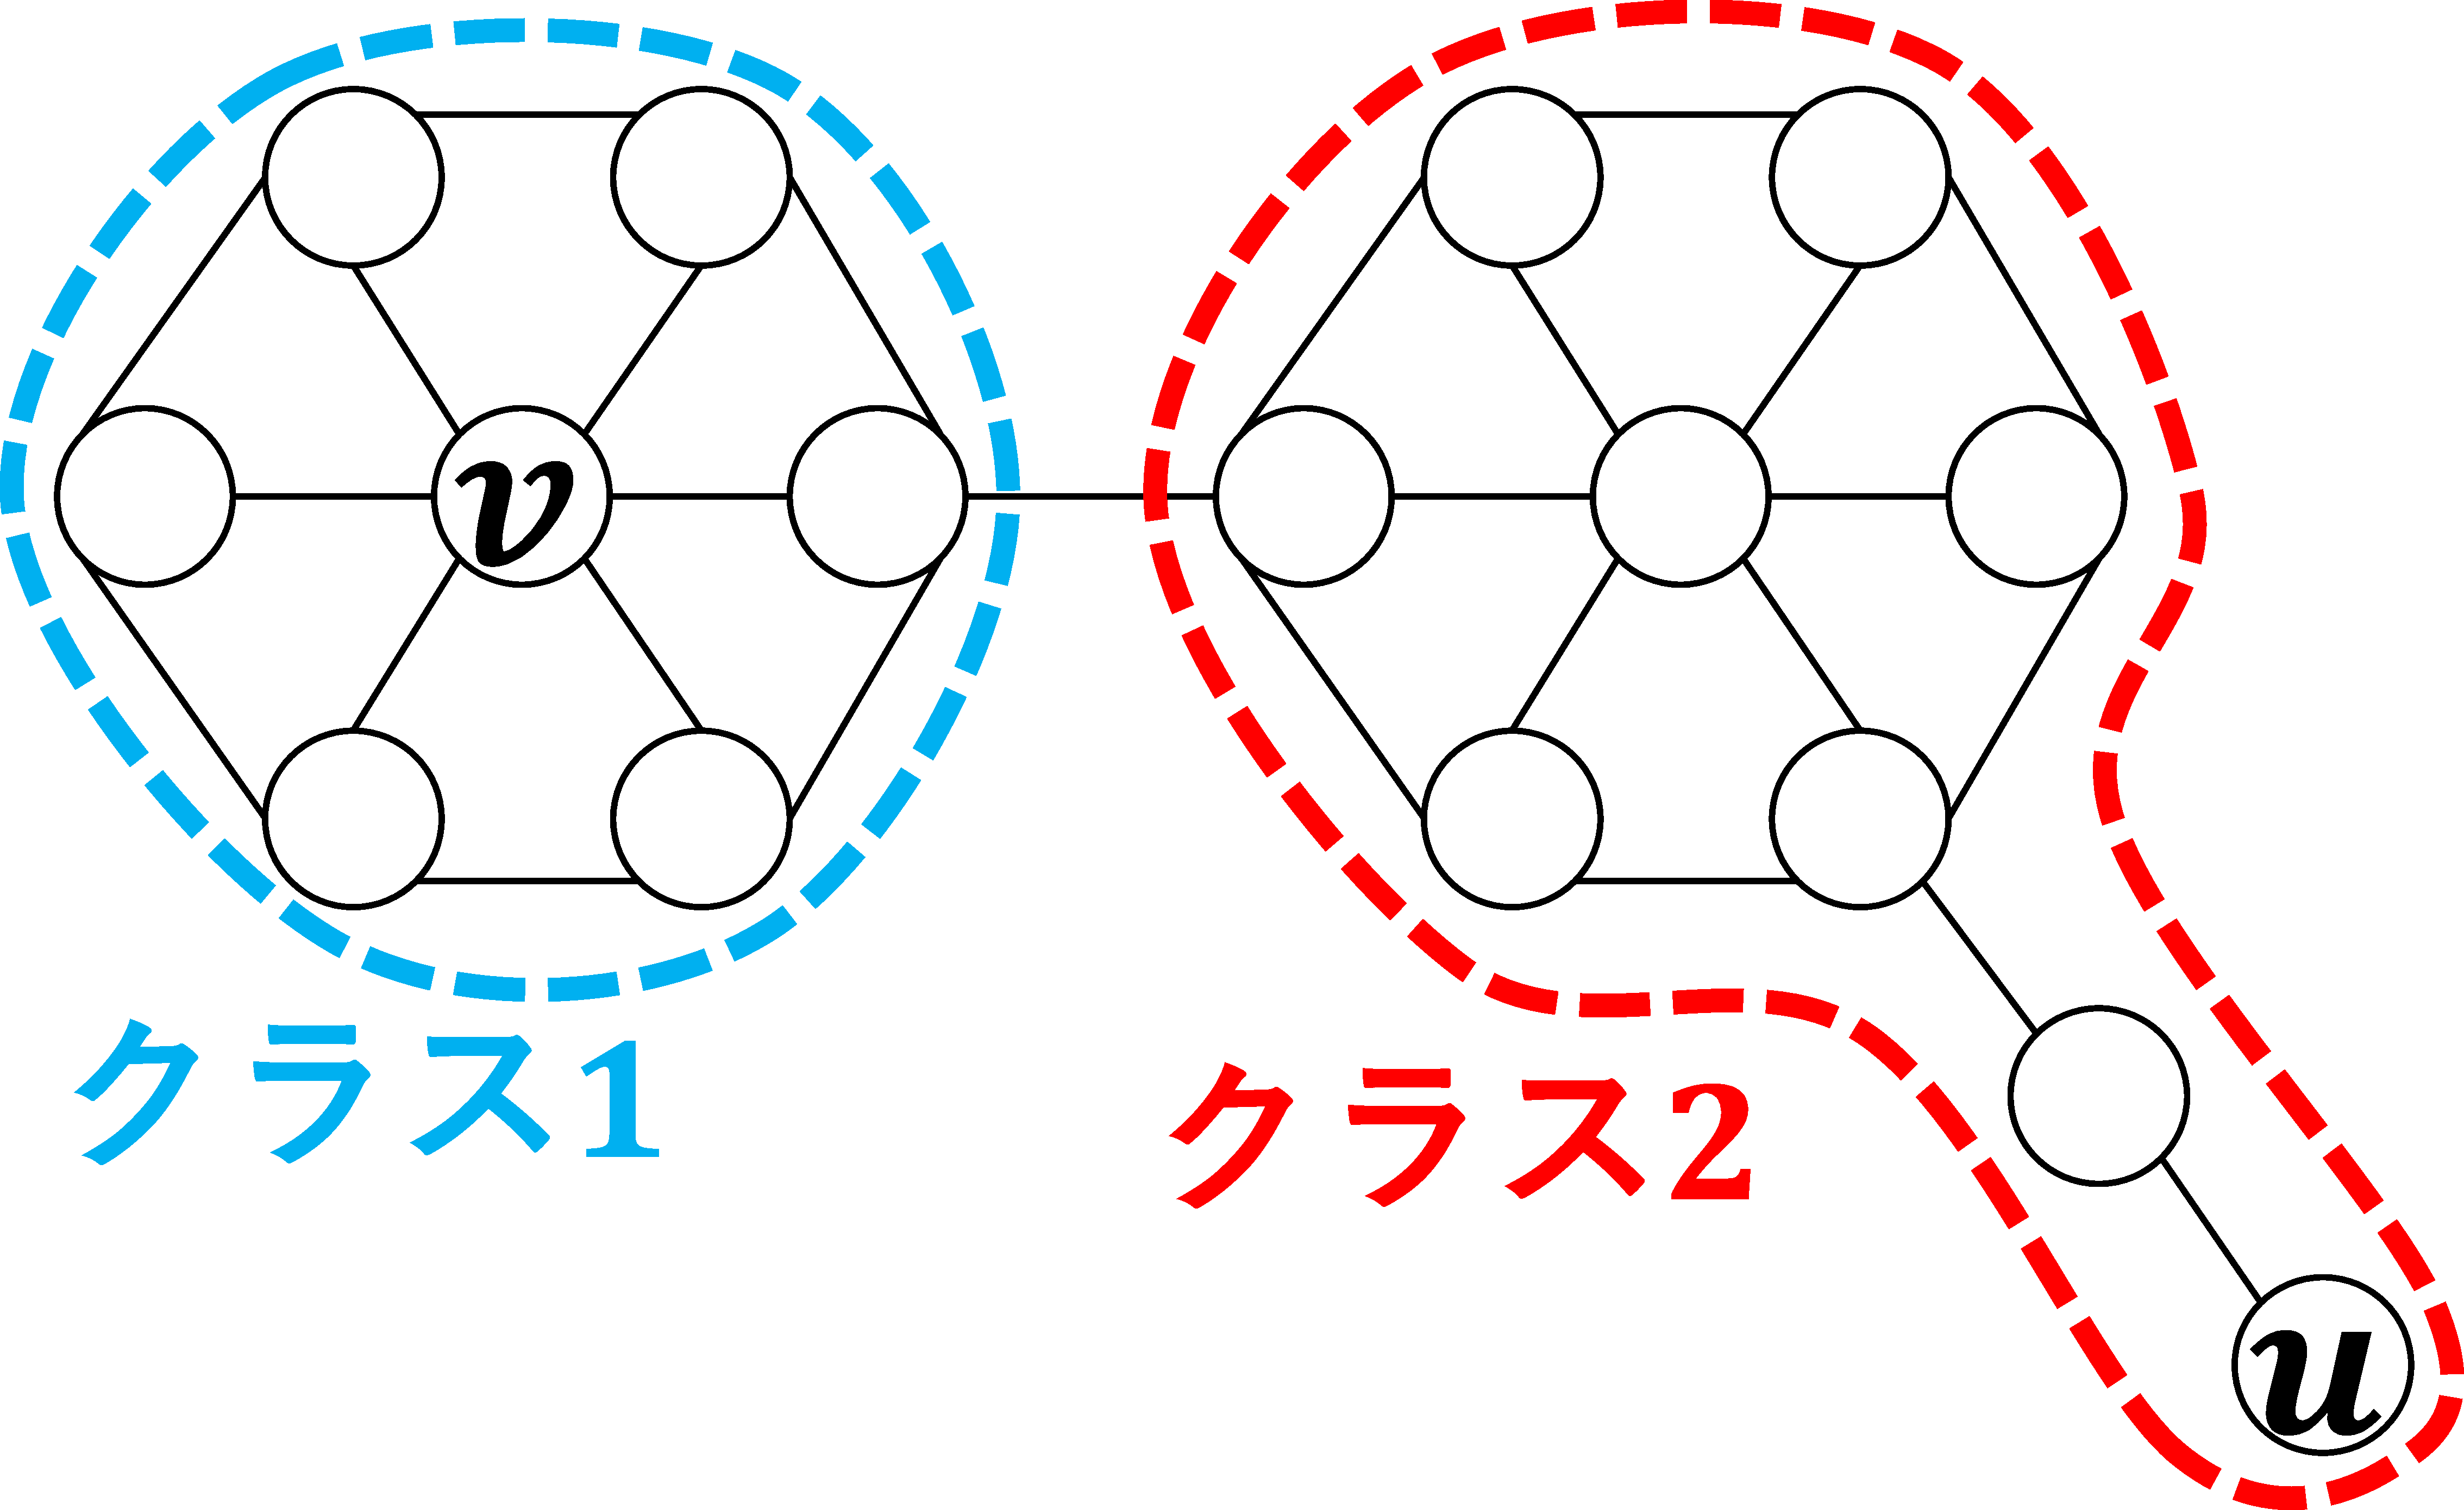
\includegraphics[height=3.6cm,width=8.5cm]{example1.pdf}
  \vspace{-6mm}
  \caption{グラフの中心にある$v$と端にある$u$}
  \label{fig_example1}
\end{figure}

\vspace{-1mm}
式(\ref{eq_gnn2})より、$L$層GNNは、どの頂点$v$についても、$L$近傍内の属性が集約された$\bm{h}_v^L$を$\bm{h}_v$として出力する。
つまり、どの頂点$v$についても、近傍の集約距離を一括して$L$としている。
よって、頂点$v$ごとに適切な集約距離$L_v^*$を学習することはできず、Over-smoothingを引き起こしている、と推察する。

%%%%%%%%%%%%%%%%%%%%%%%%%%%%%%%%%%%%%%%%
\section{提案インターフェース:Summarize-GNN}
\label{sec_proposal}

式(\ref{eq_gnn2})の代わりに、以下の$L_v^*$を学習するSummarize関数をもつ、Summarize-GNNというインターフェースを提案する。\vspace{-3mm}
\begin{align}
  & \bm{h}_v   = \text{Summarize}(\bm{h}_v^1,\ldots,\bm{h}_v^L) = \sum_{l=1}^L \alpha_v^l \bm{h}_v^l \label{eq_summarize}
\end{align}

\vspace{-2mm}
\noindent
但し、$\alpha_v^l$は学習可能パラメータであり、$\sum_{l=1}^L \alpha_v^l=1$を満たす。

式(\ref{eq_gnn1})の従来のGNNのConvを$L$回繰り返し、表現の系列$\{\bm{h}_v^1,\ldots,\bm{h}_v^L\}$を得る。
次に、式(\ref{eq_summarize})のSummarize関数に$\{\bm{h}_v^1,\ldots,\bm{h}_v^L\}$を入力し、
各表現$\bm{h}_v^l$をパラメータ$\alpha_v^l$で重み付けし、最終的な表現$\bm{h}_v$として出力する。
尚、インターフェースを提案するこの節では、$\alpha_v^l$の具体的な学習手法は述べない。

もしパラメータ$\alpha_v^l$が適切に学習できれば、図\ref{fig_example1}のグラフの中心にある頂点$v$の場合、$(\alpha_v^1,\alpha_v^2,\alpha_v^3,\alpha_v^4)=(1,0,0,0)$で、1近傍内の属性が集約されている表現$\bm{h}_v^1$に大きな重み付けができる。
一方、図\ref{fig_example1}のグラフの端にある$u$の場合、$(\alpha_u^1,\alpha_u^2,\alpha_u^3,\alpha_u^4)=(0,0,0,1)$で、より遠い4近傍内の属性が集約されている表現$\bm{h}_u^4$に大きな重み付けができる。
つまり、$\alpha_v^l$は、各$l$が頂点$v$にとって適切な集約距離$L_v^*$である確率と捉えられる。
また、この$\alpha_v^l$を学習することは、$L_v^*$を学習することに対応し、Over-smoothing防止が期待できる。


%%%%%%%%%%%%%%%%%%%%%%%%%%%%%%%%%%%%%%%%
\section{提案手法:$\alpha_v^l$の教師なし学習}
\label{sec_oversmoothing}

どのような条件を満たすとき$\alpha_v^l$が高くなるか、クラスラベルを用いずに考える。
\ref{sec_over_smoothing}節冒頭で述べたように、多層($L$層)のGNNで得られる表現$\bm{h}_v^L$は質が低い。
そこで、$\bm{h}_v^L$を反面教師と捉えて、その反面教師と$\bm{h}_v^l$間の類似度が低い、という条件を満たすとき$\bm{h}_v^l$は質が高いと考える。
つまり、$\bm{h}_v^L$と$\bm{h}_v^l$間の類似度が低いという条件を満たすとき$\alpha_v^l$が高くなると考える。

この条件が正しいことを説明するため、図\ref{fig_example2}左上で示すように、各頂点$v$が単一の属性値$x_v\in \mathbb{R}$をもつグラフの例を用いる。
属性値$x_v$の大きさは、図\ref{fig_example2}右側の横軸のように色の濃さで表す。
また、各頂点の属性$x_v$はクラスラベル$y_v$に応じたガウス分布に従うと仮定する。
例えば今回の例の場合、クラスラベルが1の頂点の属性値$x_1,x_2,x_3$は$\mathbb{G}(\mu_1, \sigma_1^2)$に、クラスラベルが2の頂点の属性値$x_4,x_5,x_6$は$\mathbb{G}(\mu_2, \sigma_2^2)$に従う。
\vspace{-1mm}

\begin{figure}[!h]
  \centering
  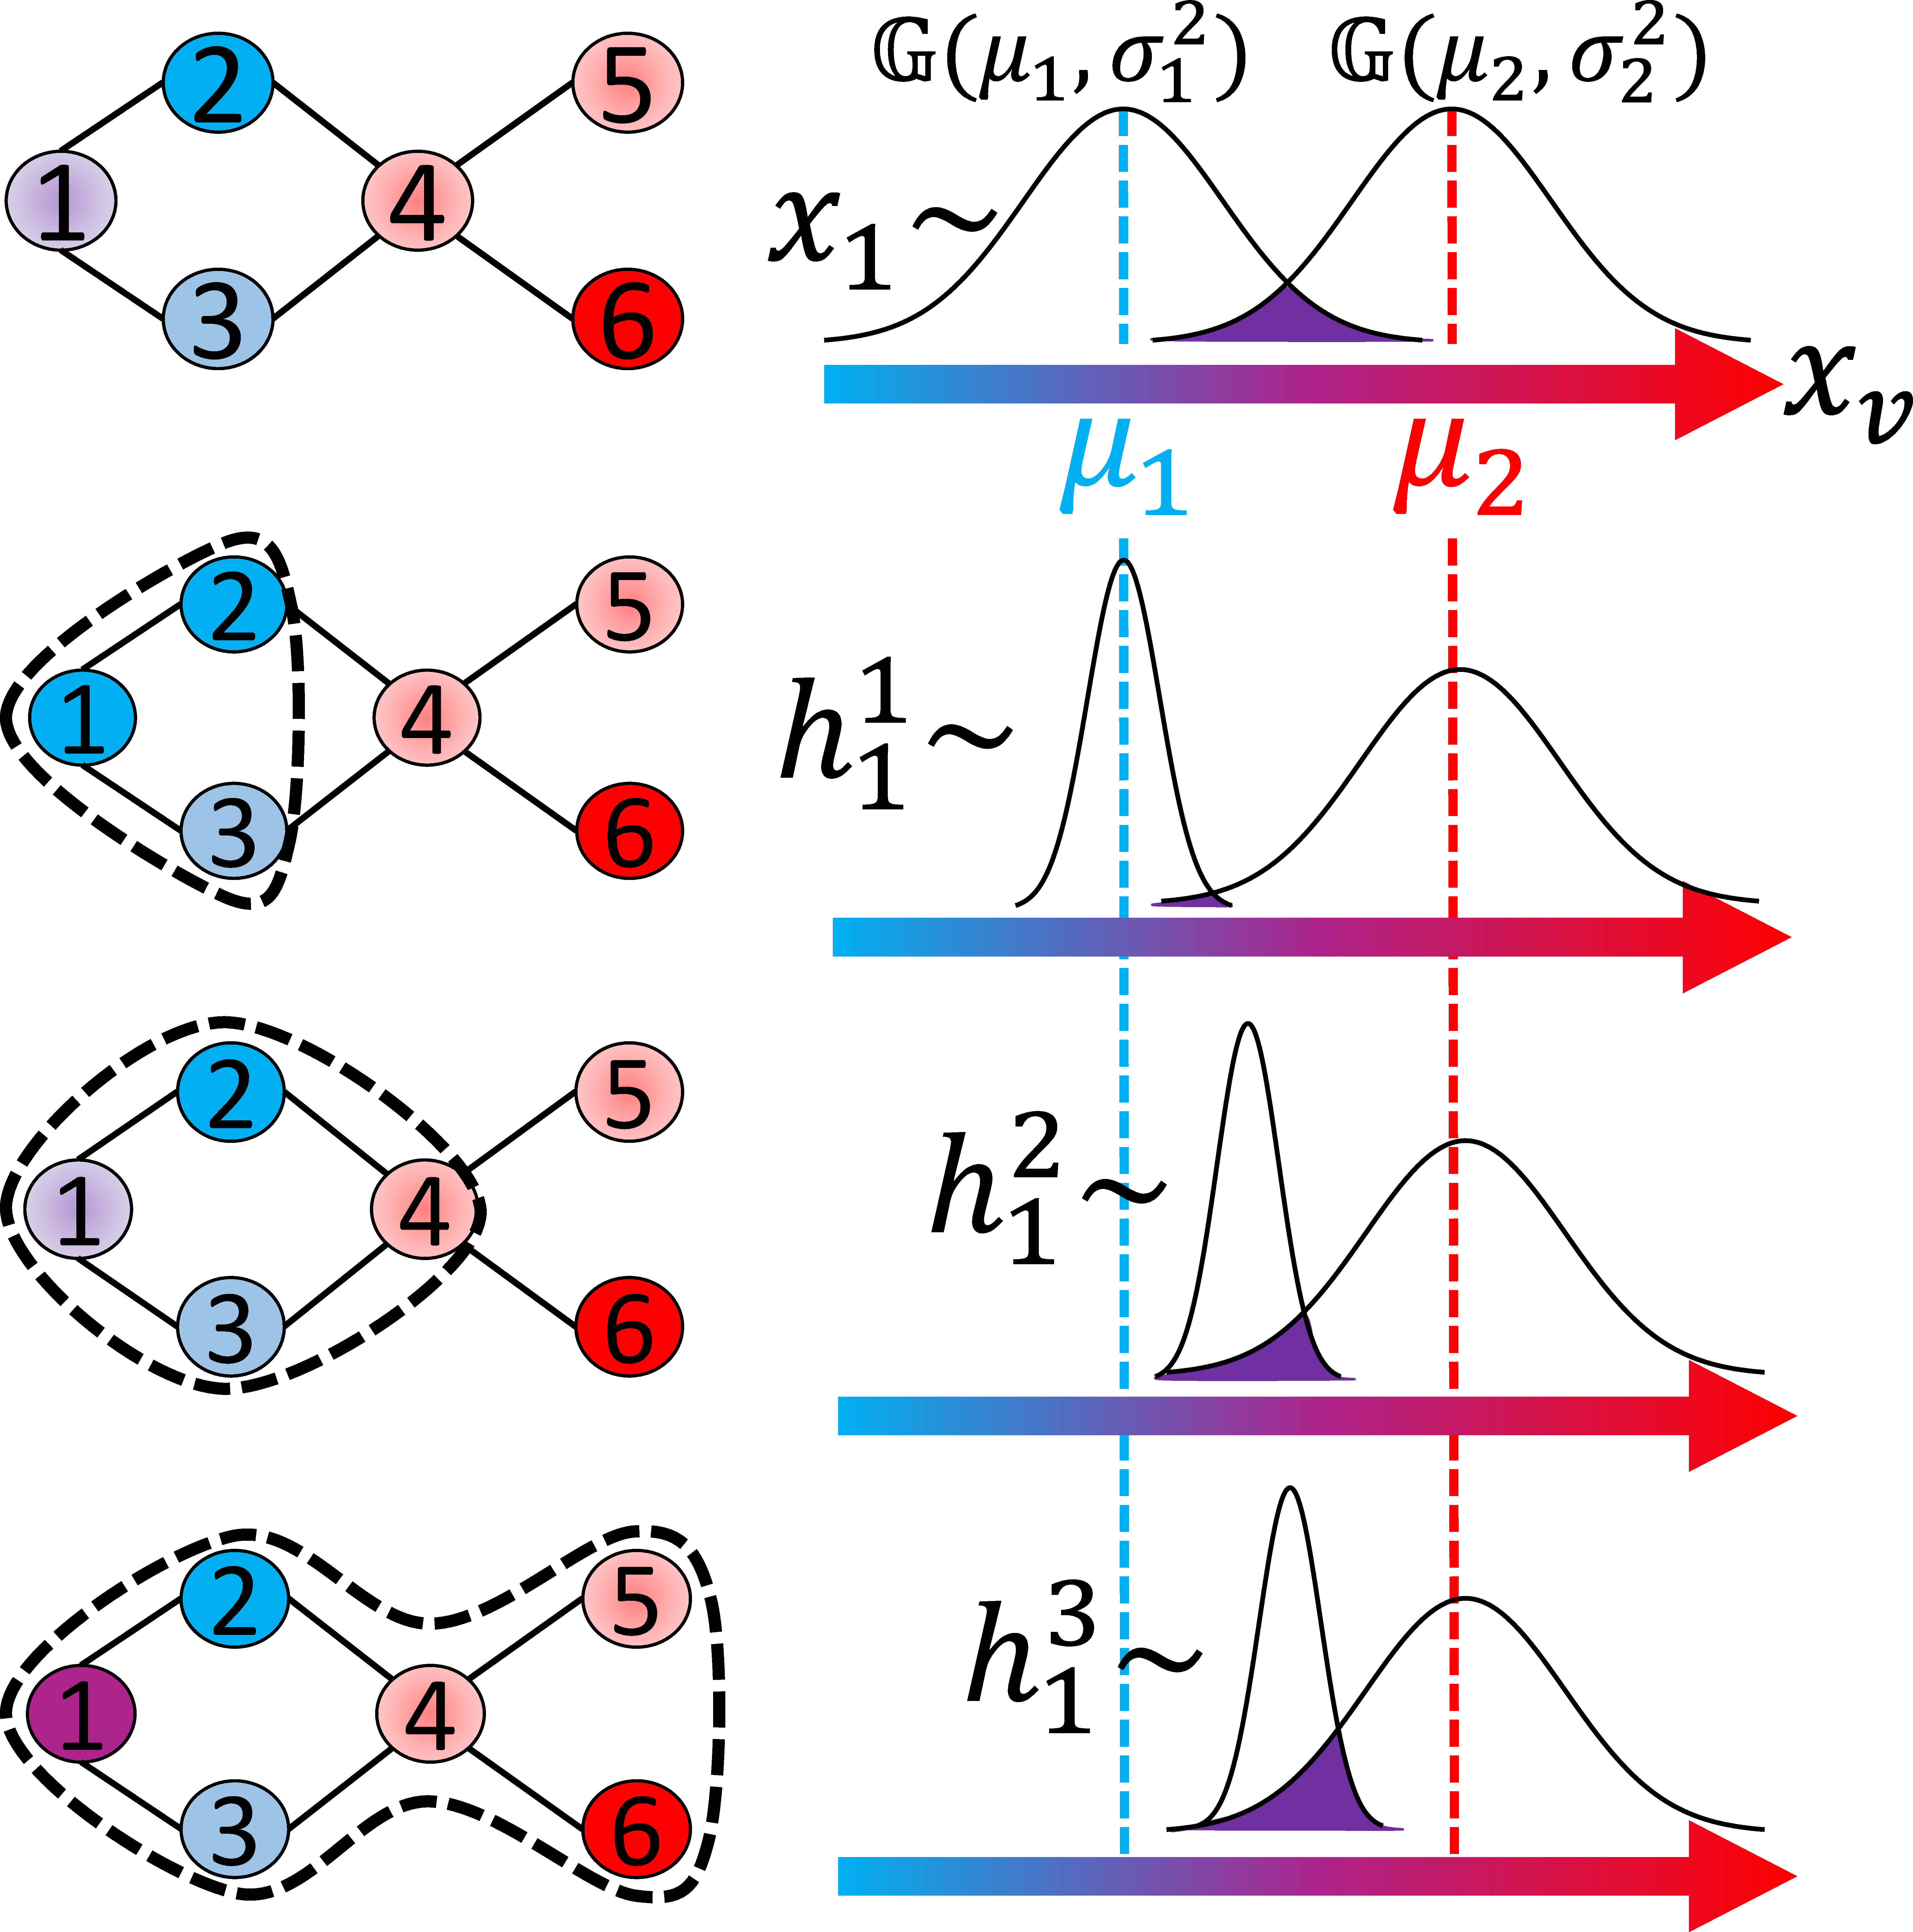
\includegraphics[height=9cm,width=9.5cm]{example2.pdf}
  \vspace{-6mm}
  \caption{グラフ$G$と、集約距離$l$により変化する$h_1^l$の従う分布}
  \label{fig_example2}
\end{figure}

\begin{comment}
  $\mathbb{G}(\mu_1, \sigma_1^2)$と$\mathbb{G}(\mu_2, \sigma_2^2)$間には、図\ref{fig_example2}右側一段目の紫色で塗りつぶした重なりがある。
図\ref{fig_example2}左側で紫色で塗り分けている頂点1の属性値$x_1$は、その重なった位置から生起しているため、クラスラベルが1か2を予測することは困難である。
つまり、分布間の重なりが大きくなる程、頂点を正しくクラス分類することは困難になる。
\end{comment}

\vspace{-2mm}
頂点のクラスラベルが全て分かっていれば、頂点1は1近傍内を集約すれば、自身と同じラベルの頂点の属性値$x_2$と$x_3$を全て集約できる。
よって$L_1^*$は1であり、最適な$(\alpha_1^{1*},\alpha_1^{2*},\alpha_1^{3*})$は$(1,0,0)$である。
対して、本研究の考える、クラスラベルが不要な条件に基づき求まる$(\alpha_1^1,\alpha_1^2,\alpha_1^3)$の期待値について考える。

層数$l=1$のGNNにより、頂点$1$には1近傍内の属性が集約、足し合わされる(図\ref{fig_example2}左側二段目)。
つまり、同じガウス分布$\mathbb{G}(\mu_1, \sigma_1^2)$に従う属性が足し合わされる。
同じ分布に従う属性を足し合わせることで得られる表現が従う分布は、元々従う分布$\mathbb{G}(\mu_1, \sigma_1^2)$と比較して、平均は維持したまま分散が小さくなる(図\ref{fig_example2}右側一段目と二段目を比較)、ということが分布の再生成という統計の性質から導ける。
\begin{comment}
  よって、分布間の重なりを減らすことができ、頂点$v$を正しくクラス分類することが期待できる。
また、このときの層数こそが、頂点$1$にとって適切な層数$L_1^*$と考える。
\end{comment}

しかし、1を超えて、2,3層と、よりGNNを多層にすると、異なるガウス分布$\mathbb{G}_2$から生起する属性も頂点$v$に足し合わされる(図\ref{fig_example2}左側三、四段目)。
すると、同じく分布の再生成という性質から、分布の平均は$\mu_1$と$\mu_2$の間にずれる。
\begin{comment}
  そのため、分布間の重なりが増え、質の低い表現を得ることが明らかになった(図\ref{fig_example2}右側二段目から三、四段目)。
\end{comment}

以上から、GNNの層数$l$を1,2,3と伸ばすに連れて、各表現$\bm{h}_1^l$の従う分布がどのように移り変わるか観察した。
$l$が1のとき、図\ref{fig_example2}右側四段目の分布から生起する質の低い反面教師$\bm{h}_1^3$と、右側二段目の分布から生起する$\bm{h}_1^1$間の類似度の期待値は低い。
よって確率$\alpha_1^1$の期待値は高い。
一方、$l$が2のとき、$\bm{h}_1^3$と、右側三段目の分布から生起する$\bm{h}_1^2$間の類似度の期待値は高い。
よって確率$\alpha_1^2$の期待値は低い。

以上の例を用いて、本研究が提案する類似度に基づいた条件により、教師ラベルを用いることなく、最適($\alpha_v^{l*}$)に近い$\alpha_v^l$を求められることを説明した。
また、類似度に基づいた$\alpha_v^l$の学習手法は以下で具体的に求める。
\begin{align}
  & \overline{\alpha}_v^l = \text{Attention}(\bm{h}_v^l, \bm{h}_v^L) \label{eq_alpha_unnormalized} \\
  & \alpha_v^l = \text{Softmax}(\overline{\alpha}_v^l, L) = \frac{\exp(\overline{\alpha}_v^l)}{\sum_{l'=1}^L \exp(\overline{\alpha}_v^{l'})} \label{eq_alpha_normalized}
\end{align}
式(\ref{eq_alpha_unnormalized})のAttention\cite{Vaswani}により$\bm{h}_v^l$と$\bm{h}_v^L$間の類似度を求め、式(\ref{eq_alpha_normalized})のSoftmax関数で$\sum_{l=1}^L \alpha_v^l=1$を満たすよう正規化する。


%%%%%%%%%%%%%%%%%%%%%%%%%%%%%%%%%%%%%%%%
\section{評価実験}
\label{sec_experiment}

3つの既存モデルと提案モデルの、Over-smoothingの防止性能について比較する。
1つ目は\ref{sec_gnn}節で紹介したGNNとする。
2つ目は、式(\ref{eq_gnn1})の各ConvをSkipすることが可能なSkip-GNNとする。
3つ目は、本研究と同じ目的の下、メモリ量を要するモデルを用いて$\alpha_v^l$を学習するComplex~Summarize-GNN~(CS-GNN)とする。
類似度に基づき$\alpha_v^l$を求める本提案モデルは、CS-GNNと異なり省メモリなため、Simple~Summarize-GNN~(SS-GNN)とする。

データセット(グラフ$G$)は、PubMed,Arxiv,Reddit,PPI,$\text{PPI}_{\text{Ind.}}$の5つを用いる(頂点数は数十万)。
$G$と教師ラベル集合$Y_{train}$を用いて、各モデルを学習する。次に、残りの頂点のラベル集合$Y_{test}$の内、学習済みモデルにより正しくラベルを予測できた割合を頂点の分類精度とする。

$L$が$6\sim 8$層、つまり多層の各モデルによる分類精度を表\ref{table_pubmed}に示す。
多層にしても(層数$L$が大きくても)、精度が高いモデル程、Over-smoothingの防止性能が高いといえる。
全てのデータセットにおいて既存より同等以上のOver-smoothingの防止性能をSS-GNNは達成した。
また、他モデルよりメモリ量を要するCS-GNNがOOMに陥り実験できなかったが、SS-GNNは全データセットで実験できた。

\begin{table}[!h]
  \caption{多層な各モデルによる分類精度(*OOMはOut~of~Memory)}
  \vspace{-1mm}
  \begin{tabular}{|l|l|l|l|l|l|}
  \hline
  \multicolumn{1}{|c|}{} & \multicolumn{1}{c|}{Reddit} & \multicolumn{1}{c|}{Arxiv} & PubMed        & PPI           & $\text{PPI}_{\text{Ind.}}$ \\ \hline
  GNN                    & 79.5                        & 70.9                       & 76.8          & 81.0          & 47.9                       \\ \hline
  Skip-GNN               & 95.1                        & 71.2                       & 86.8          & 81.5          & 97.7                       \\ \hline
  CS-GNN                 & OOM*                         & OOM*                        & 88.8          & 80.8          & \textbf{99.1}              \\ \hline
  SS-GNN                 & \textbf{96.5}               & \textbf{72.7}              & \textbf{89.4} & \textbf{82.1} & \textbf{99.0}              \\ \hline
  \end{tabular}
\end{table}


%%%%%%%%%%%%%%%%%%%%%%%%%%%%%%%%%%%%%%%%
\section{まとめ}
GNNの課題であるOver-smoothingを防止するべく、頂点$v$ごとの適切な集約距離$L_v^*$を学習するSS-GNNを提案した。
既存モデルGNN,Skip-GNN,CS-GNNと比較して、SS-GNNは同等以上のOver-smoothing防止性能を持ちつつ、大規模データセットにも適用可能なモデルであることが実験的に示された。


%%%%%%%%%%%%%%%%%%%%%%%%%%%%%%%%%%%%%%%%

\bibliographystyle{jplain}
\renewcommand{\bibname}{参考文献}
\begin{thebibliography}{1}
\addcontentsline{toc}{chapter}{参考文献}
\markboth{参考文献}{参考文献}
\vspace{-2mm}

\bibitem{Kipf}
T. N. Kipf, M. Welling.:
Semi-supervised classification with graph convolutional networks,
{\it arXiv Preprint}, arXiv:1609.02907 (2016).
\vspace{-0.3mm}

\bibitem{Velickovic}
P. Veli{\v{c}}kovi{\'c}, et al.:
Graph attention networks,
{\it arXiv Preprint}, arXiv:1710.10903 (2017).
\vspace{-0.3mm}

\bibitem{Vaswani}
A. Vaswani, et al.:
Attention is all you need,
{\it NIPS}, pp.~5998--6008 (2017).
\vspace{-0.3mm}

\bibitem{Li}
G. Li, et al.:
Deepergcn: All you need to train deeper gcns,
{\it arXiv Preprint}, arXiv:2006.07739 (2020).
\vspace{-0.3mm}

\bibitem{Xu1}
K. Xu, et al.:
Representation learning on graphs with jumping knowledge networks,
{\it ICML}, pp.~5453--5462. PMLR (2018).
\vspace{-0.3mm}

\end{thebibliography}
\end{document}